\documentclass[12pt]{article}
\usepackage{graphics}
% \usepackage{subfigure}
\usepackage{times}
\usepackage{mathptmx}
\usepackage[margin=2cm]{geometry}

\usepackage[usenames,dvipsnames]{xcolor}
\usepackage[colorlinks=true,linkcolor=black,citecolor=BlueViolet,urlcolor=Maroon]{hyperref}
\usepackage{subcaption}
\usepackage{enumerate}
\usepackage{amsthm, amsmath, amssymb} % Mathematical typesetting

\usepackage{tikz}

\title{Towards more accurate fingerprint recognition using minutiae feature graph}
\author{Feng Yulin, 18070069r\\Cao Pei, }
\date{\today}

\linespread{1}

\begin{document}

\maketitle

\begin{abstract}
    This paper
\end{abstract}
\section{Introduction}

Fingerprint recognition is an increasingly popular research domain of research and has attracted significant attention from both the academia and industry.
It is one of the most accurate and reliable human biometrics recognition technology, and has been widely used in a great many of civilian applications such as forensics, e-business application, physical access control, large-scale identifications applications, etc \cite{finger-handbook}.

Generally speaking, the fingerprint images can be classified as 3 categories: plain, latent and rolled \cite{nimkarFingerprintSegmentationAlgorithms2014}.
The plain fingerprint images are usually acquired by touching the fingers on a flat surface.
The latent images are usually collected from some real crime scenes, therefore is usually low quality and contains a lot of noise.
And the rolled fingerprint images are often collected by rolling the fingers from one side to another, which can keep most of the fingerprint ridge information \cite{nimkarFingerprintSegmentationAlgorithms2014}.
There are seven kinds of main factors which is responsible for the intra-class variations:  displacement, rotation, partial overlap, non-linear distortion, press and skin condition,  noise and feature extraction errors \cite{finger-handbook}.
The most important and difficult factor is the  non-linear distortion problem. This kind of error is generated on the process of sensing  the 3D fingerprint shapes into a 2D flat surface. Most fingerprint matching algorithms  usually do not consider such variations, and consider the obtained fingerprint images  as non-distorted by assuming that it was produced by a correct finger placement.  Fingerprint recognition can be divided into two parts: fingerprint segmentation and  fingerprint matching. Fingerprint segmentation is the process which extract the  foreground regions from the original fingerprint images \cite{finger-handbook}. There are many different  kinds of segmentation methods and in this survey and project, we will use segmented  images and will only concentrate on the matching part. In the following survey details  part, we will introduce some newly published deep learning-based fingerprint  recognition algorithms.  
\section{Related Work}

\section{Methodology (Research Project Details)}


\subsection{Minutiae Extraction}


\begin{figure}[htbp]
    \centering
    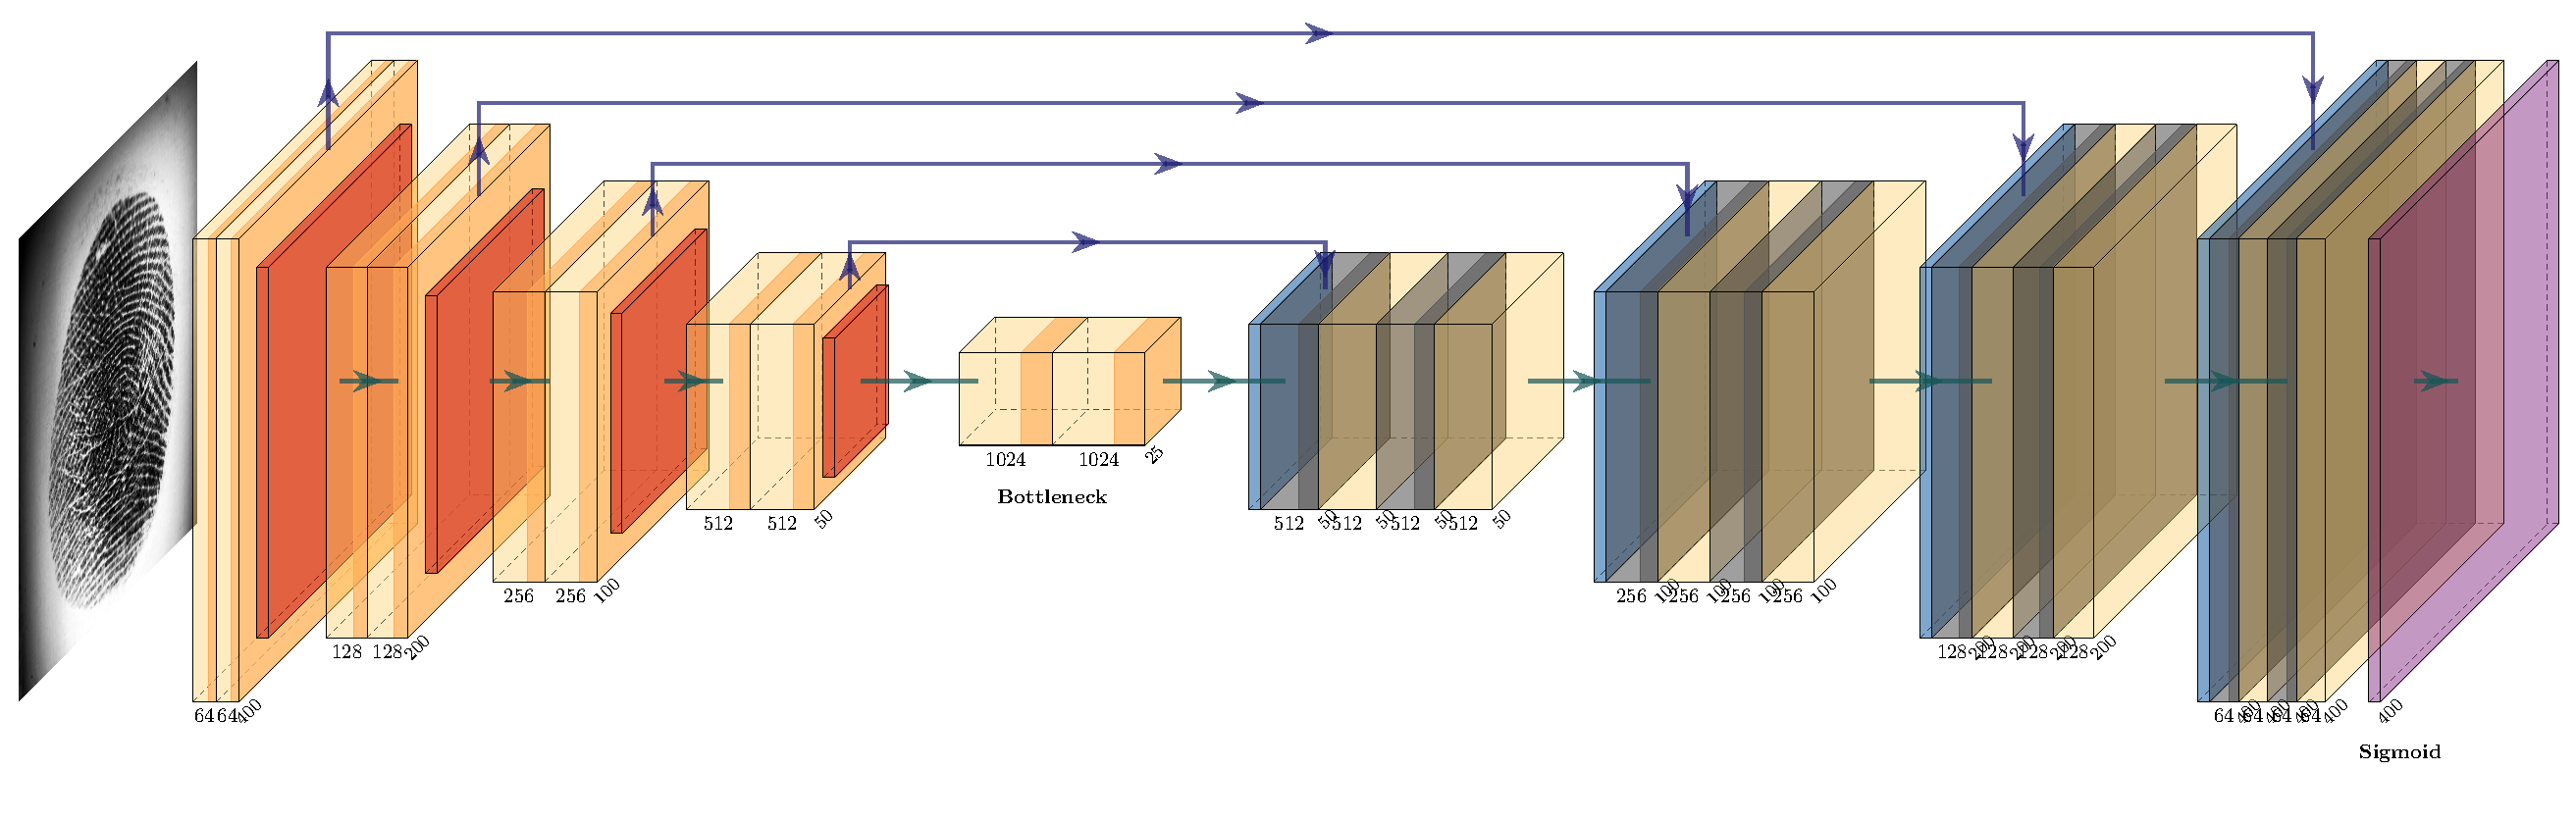
\includegraphics[width=.9\linewidth]{fig/unet.pdf}
    \caption{The structure of our minutiae feature neural network, generated with \cite{PlotNeuralNet}}
    \label{fig:unet}
\end{figure}

Fig. \ref{fig:unet} presents the basic structure of our minutiae detection network.
We input the augmented fingerprint images (with a size of $ 560*400 $ ) into the neural network and then use a UNet to extract the minutiae from it.
We use the ResNet18 as encoder or backbone and use pre-trained weights in imagenet for the backbone initialization.


\subsection{Minutiae Feature}


\subsection{Minutiae Graph Matching}


\subsection{Loss Function}


\subsection{Data Augmentation}

\begin{figure}[htbp]
    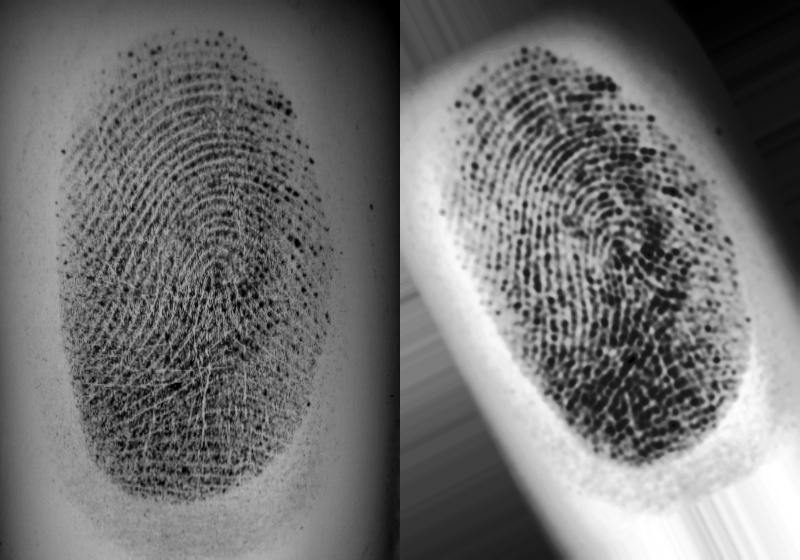
\includegraphics[width=.32\linewidth]{fig/augmentation/aug-1.jpg}
    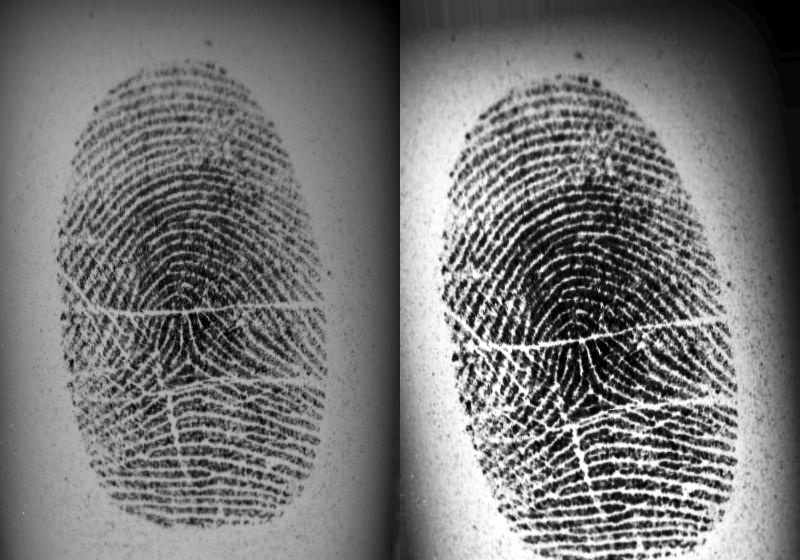
\includegraphics[width=.32\linewidth]{fig/augmentation/aug-2.jpg}
    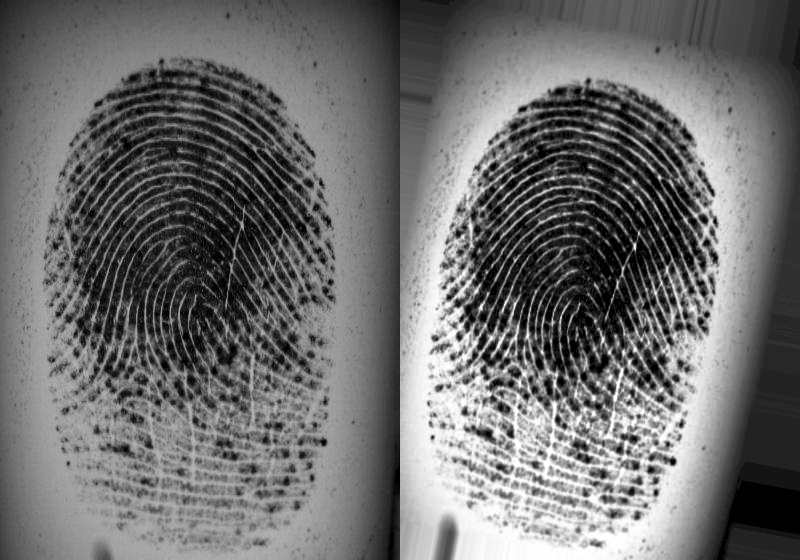
\includegraphics[width=.32\linewidth]{fig/augmentation/aug-3.jpg}
    \newline
    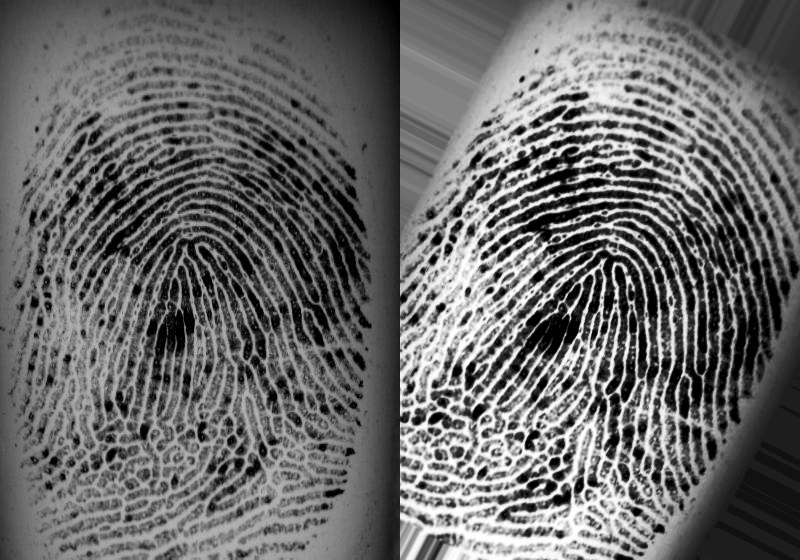
\includegraphics[width=.32\linewidth]{fig/augmentation/aug-4.jpg}
    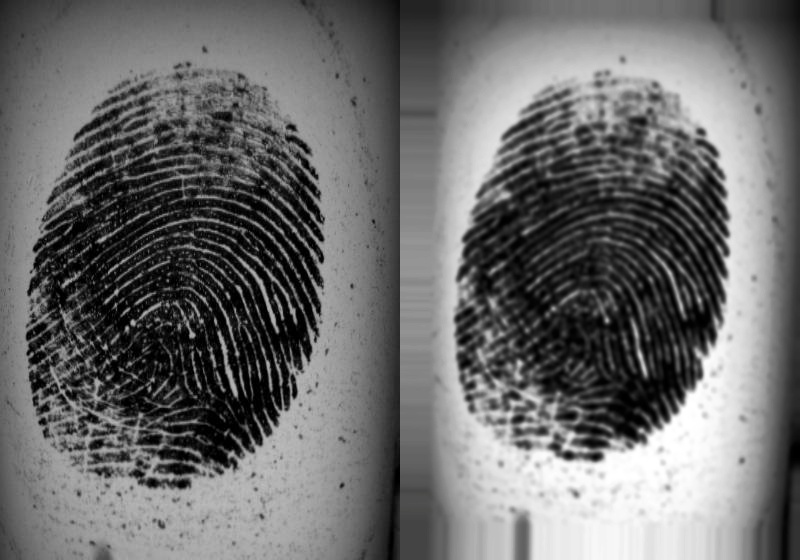
\includegraphics[width=.32\linewidth]{fig/augmentation/aug-5.jpg}
    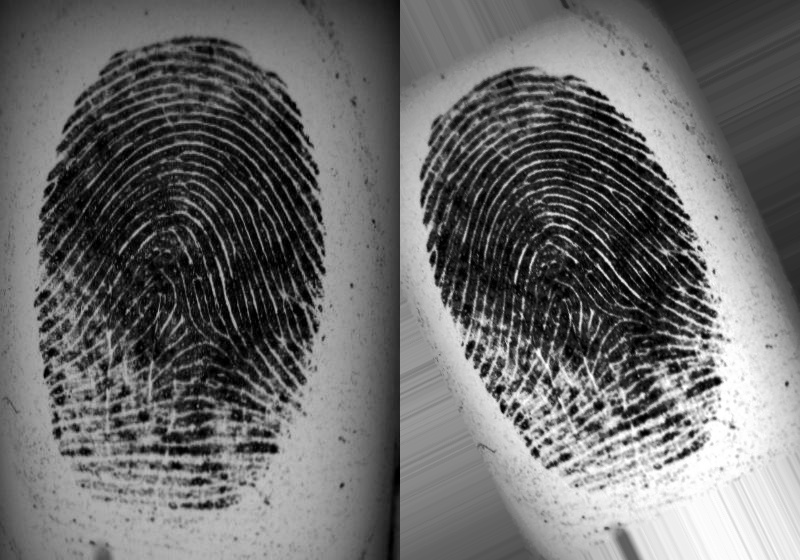
\includegraphics[width=.32\linewidth]{fig/augmentation/aug-6.jpg}
    \caption{Augmentation images samples, left are the original images while right are the augmented images}
    \label{fig:augmentation}
\end{figure}

It is worth to mention that we also do some data augmentation in our experiment to improve the robustness and accuracy.
We use imgaug \cite{imgaug} library in this experiment.
And mainly use the following transforms: random brightness, gamma contrast, Gaussian blur and shift scale rotate.
After the data augmentation, we add a histogram equalization to normalize the images.
Fig \ref{fig:augmentation} presents some sample data augmentation images pairs, where the left is the original fingerprint image and the right is the augmented image.



\section{Experiments and Results}

\subsection{Training Data Preparation}

\begin{figure}[htbp]
    \centering
    \subcaptionbox{Minutiae detected by NBIS (with a high quality threshold)\label{subfig:NBIS-high}}{
        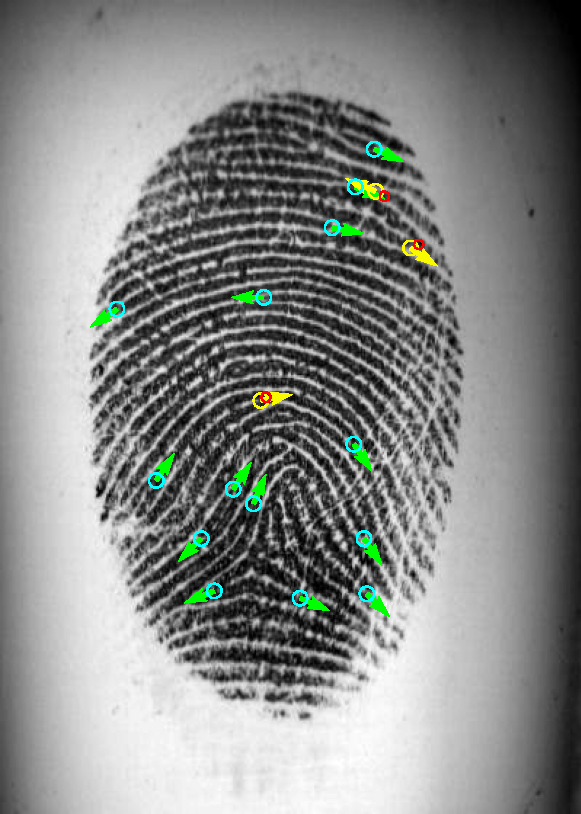
\includegraphics[width=.3\linewidth]{fig/label/nbis-high-thre.pdf}
    }
    \quad
    \subcaptionbox{Our manually marked minutiae\label{subfig:manually-label}}{
        \includegraphics[width=.3\linewidth]{fig/label/manually.png}
    }
    \quad
    \subcaptionbox{Minutiae detected by NBIS (with a low quality threshold)\label{subfig:NBIS-low}}{
        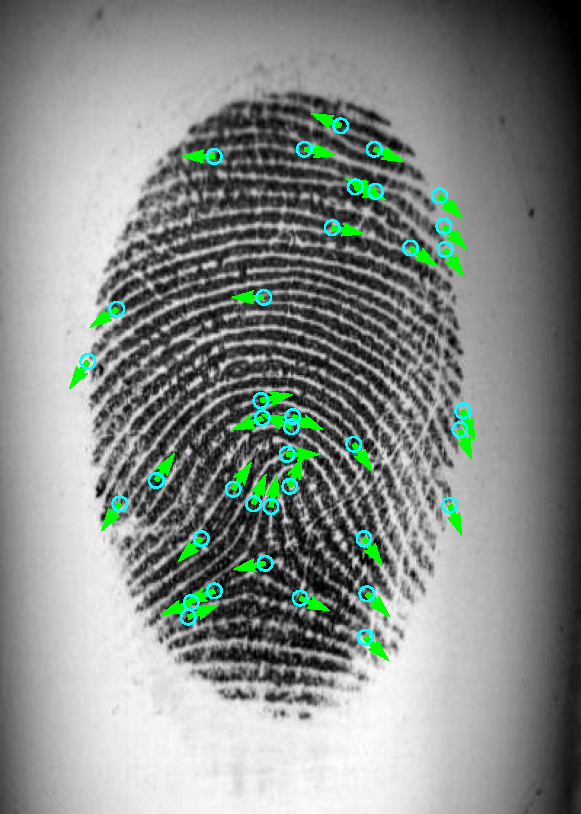
\includegraphics[width=.3\linewidth]{fig/label/nbis-low-thre.pdf}
    }
    \caption{A sample manually marked minutiae with corresponding NBIS detected minutiae}
    \label{fig:label}
\end{figure}


We first tried to use NBIS \cite{NBIS} to mark the ground truth minutiae and use it for training.
However, we found that the minutiae detection accuracy of NBIS is low.
It will output an image quality number together with the minutiae location and we can set a threshold to select minutiae.
However, the accuracy is low and if we set a high threshold, then many correct minutiae could not be detected, such as the image shown in Fig. \ref{subfig:NBIS-high}.
And if we set a higher threshold, then it will detect many wrong minutiae, as shown in Fig. \ref{subfig:NBIS-low}.
Besides, it cannot find an accurate minutiae threshold, as it either detected a lot of wrong minutiae or miss many important minutiae, or both.
In addition, the locations of much minutiae were wrongly labeled.
For example, in Fig. \ref{subfig:NBIS-low}, three minutiae's locations was not correct and we highlight them using yellow color, and we also mark the correct position with red circle.
We can find that there are about 10 pixels gap between the correct minutiae location and those wrongly detected minutiae location, which will make it harder to train a good model.

Therefore, we decide to mark the ground truth minutiae ourselves using labelme \cite{labelme}.
Because it is difficult to find some latent minutiae in the original image, we first enhance the original fingerprint image by estimating the orientation first and then binarizing with the orientations \cite{caoFingerprintImageEnhancement2017}.
After that, we merge the binarized enhanced images with the original images, and then use labelme to manually mark the minutiae on the merged images.
We did not directly use the binarization enhanced images because that there are much wrong minutiae in the enhanced images, therefore we should refer the original images too.
Fig. \ref{subfig:manually-label} presents an example of the the merged images and our manually marked minutiae.
It is the same image as Fig. \ref{subfig:NBIS-low} and \ref{subfig:NBIS-high}, where our manually marked minutiae is much more accurate than them.

As a result, we first manually selected 200 fingerprint images from the FVC2006 dataset \cite{FVC2006} and marked them manually.
Because we thought these images were not enough and therefore we also manually selected 300 more different high quality fingerprint images which minutiae detection are relatively accurate.
These images are all very clear and the most minutiae was detected by minutiae.
We set a high threshold (35) to filter the incorrect minutiae and get the ground truth minutiae (although there was some missed minutiae and little wrongly detected minutiae).


\subsection{Minutiae Detection}

\def\subwidth{.3}

\begin{figure}[htbp]
    \centering
    \begin{minipage}{.48\linewidth}
        \subcaptionbox{
            original image
        }{
            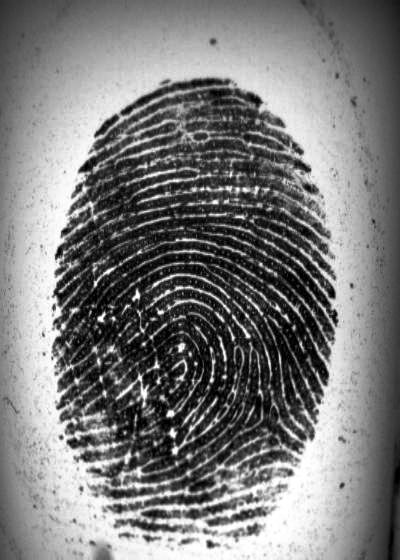
\includegraphics[width=\subwidth\linewidth]{fig/mask/ori-0.png}
        }
        \subcaptionbox{
            minutiae map
            \label{subfig:not-good-1}
        }{
            
\includegraphics[width=\subwidth\linewidth]{fig/mask/mask-0.png}
        }
        \subcaptionbox{
            merged image
        }{
            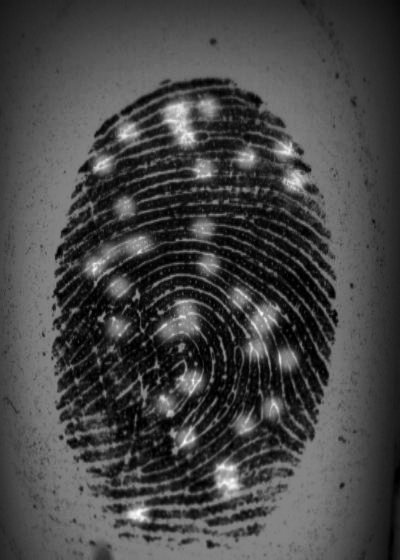
\includegraphics[width=\subwidth\linewidth]{fig/mask/merge-0.png}
        }
    \end{minipage}
    \quad
    \begin{minipage}{0.48\linewidth}
        \subcaptionbox{
            original image
        }{
            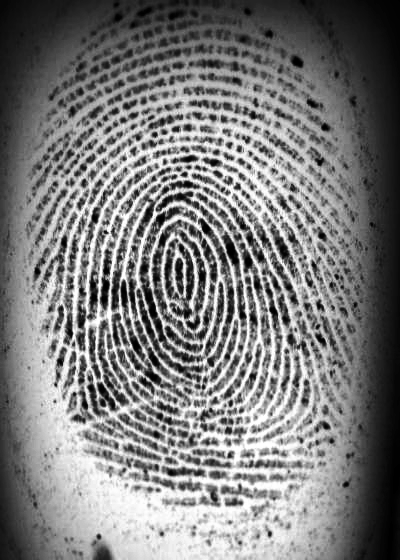
\includegraphics[width=\subwidth\linewidth]{fig/mask/ori-1.png}
        }
        \subcaptionbox{
            minutiae map
        }{
            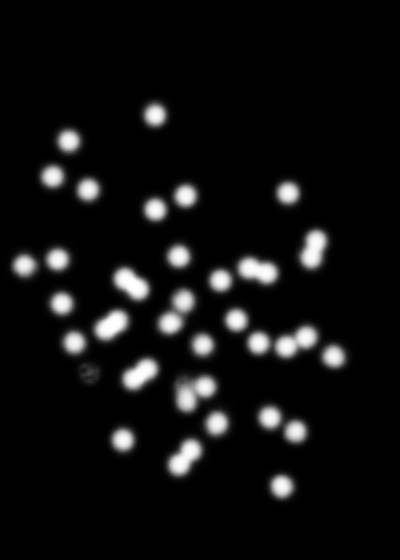
\includegraphics[width=\subwidth\linewidth]{fig/mask/mask-1.png}
        }
        \subcaptionbox{
            merged image
            \label{subfig:good-1}
        }{
            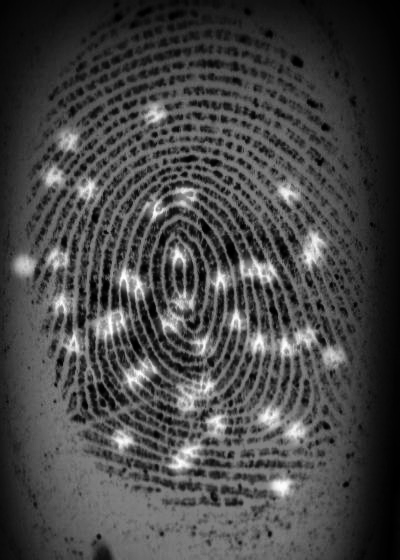
\includegraphics[width=\subwidth\linewidth]{fig/mask/merge-1.png}
        }
    \end{minipage}
    \newline
    \begin{minipage}{.48\linewidth}
        \subcaptionbox{
            original image
        }{
            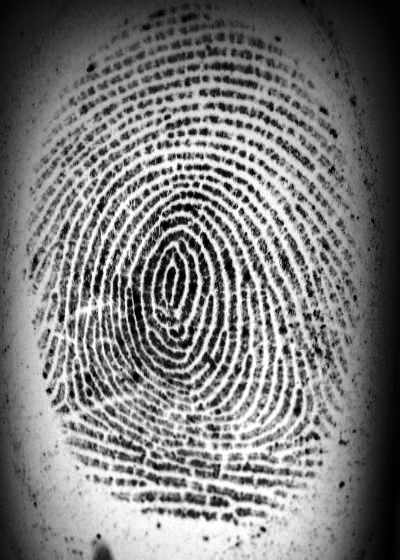
\includegraphics[width=\subwidth\linewidth]{fig/mask/ori-2.png}
        }
        \subcaptionbox{
            minutiae map
            }{
            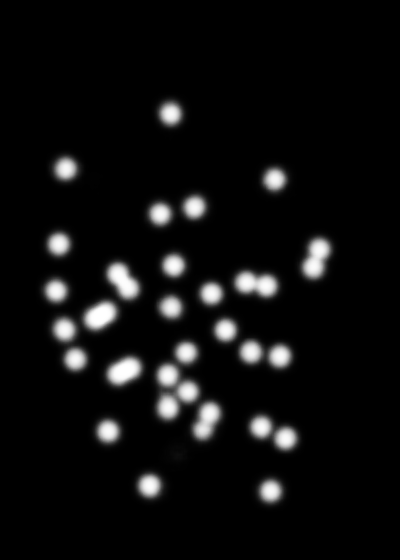
\includegraphics[width=\subwidth\linewidth]{fig/mask/mask-2.png}
        }
        \subcaptionbox{
            merged image
            \label{subfig:good-2}
        }{
            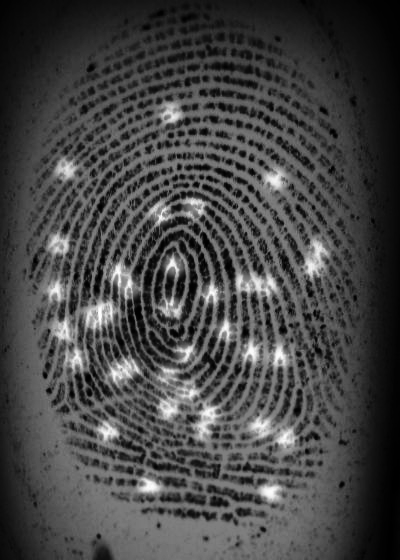
\includegraphics[width=\subwidth\linewidth]{fig/mask/merge-2.png}
        }
    \end{minipage}
    \quad
    \begin{minipage}{0.48\linewidth}
        \subcaptionbox{
            original image
        }{
            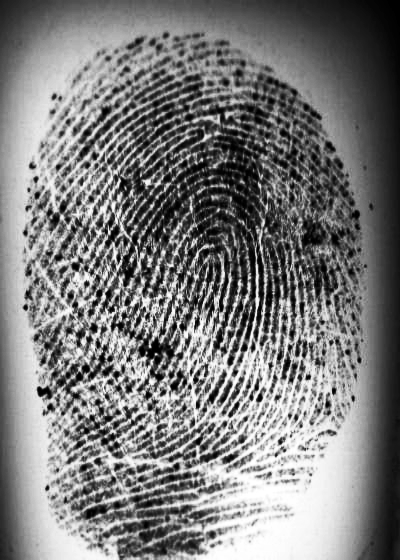
\includegraphics[width=\subwidth\linewidth]{fig/mask/ori-3.png}
        }
        \subcaptionbox{
            minutiae map
        }{
            
\includegraphics[width=\subwidth\linewidth]{fig/mask/mask-3.png}
        }
        \subcaptionbox{
            merged image
            \label{subfig:not-good-2}
        }{
            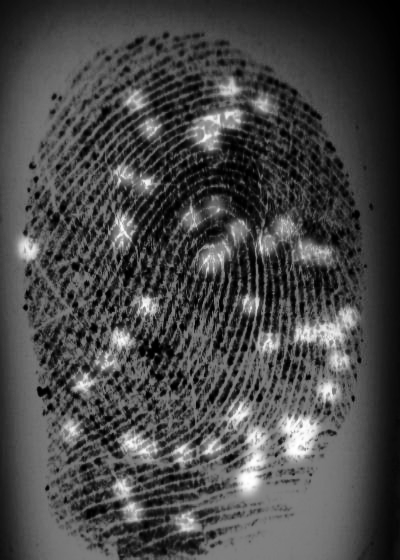
\includegraphics[width=\subwidth\linewidth]{fig/mask/merge-3.png}
        }
    \end{minipage}

    \caption{Some sample images and predicted minutiae map}
    \label{fig:minutiae-map}
\end{figure}

We test our model using the rest of the fingerprint images in FVC2006 dataset.
Fig \ref{fig:minutiae-map} presents some randomly selected sample images and corresponding minutiae map.
We also merge the original images and the predicted minutiae map to make it more clear to view.
From Fig. \ref{fig:minutiae-map}, we can find that the minutiae in sub-figure \ref{subfig:good-1} and \ref{subfig:good-2} are very accurate.
Almost every minutiae is detected and there is not wrongly detected minutiae.
The minutiae in \ref{subfig:not-good-1} and \ref{subfig:not-good-2} is a little worse, where a few minutiae in the noisy area is wrongly detected.

The minutiae detection results are much better than existing algorithms, such as MinutiaeNet \cite{MinutiaeNet}.
We used the source code provided in \cite{MinutiaeNet} and calculate the corresponding minutiae.
Fig. \ref{fig:minutiaenet-results} presents some sample minutiae detection results.
We can easily find that there is a lot of wrongly detected minutiae and missed minutiae.
Due to the time limitation, we did not implement other deep learning based algorithms and make comparison, but based on the detection results, we think our minutiae detection network achieve a very high accuracy and may surpass many existing minutiae detection algorithms.
% , therefore we refer the minutiae detection results in the papers and make a simple comparison.

\def \figwidth {.19}
\begin{figure}[htbp]
    \centering
    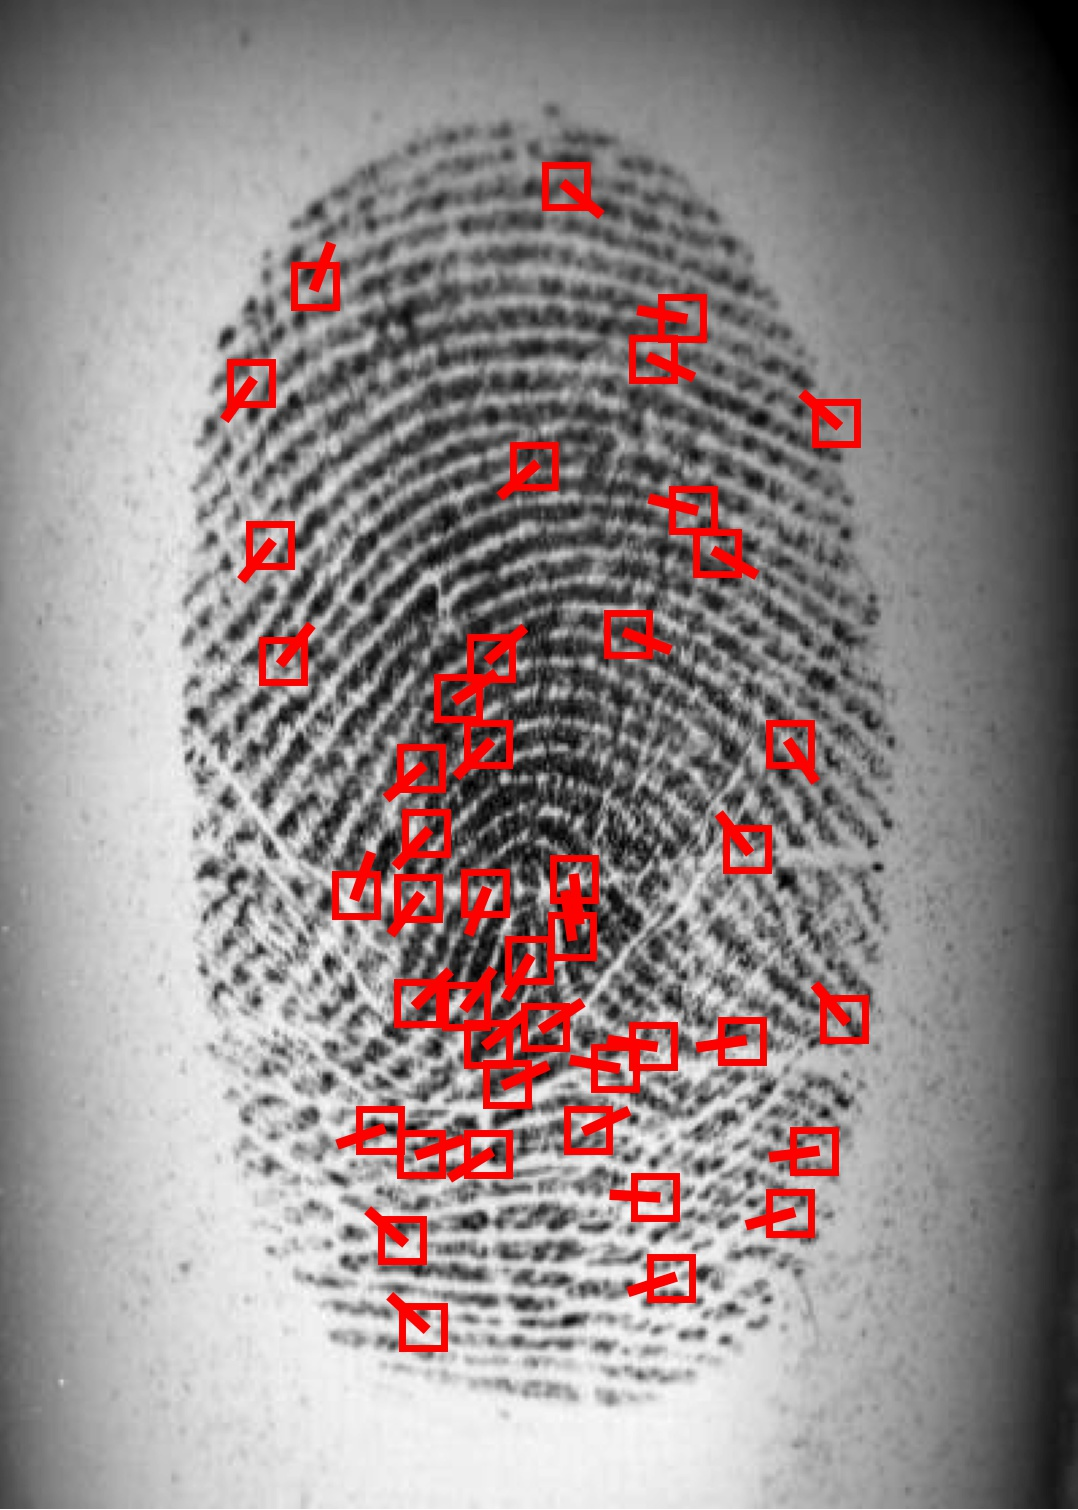
\includegraphics[width=\figwidth\linewidth]{fig/minutiaenet/1.jpg}
    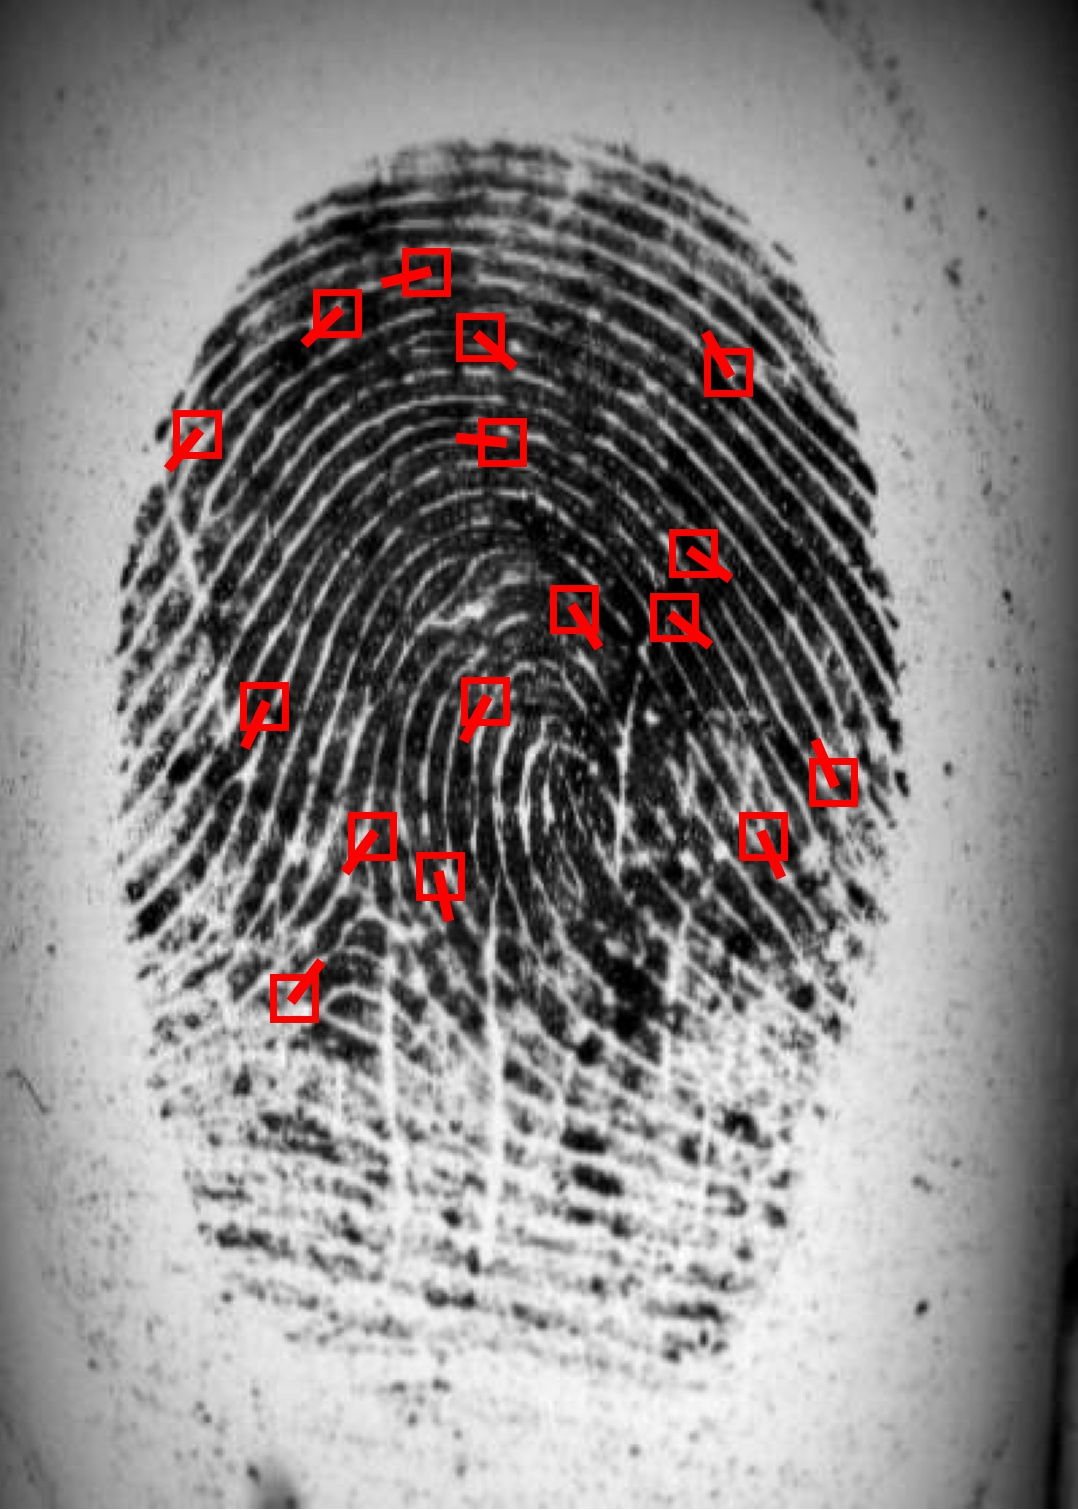
\includegraphics[width=\figwidth\linewidth]{fig/minutiaenet/2.jpg}
    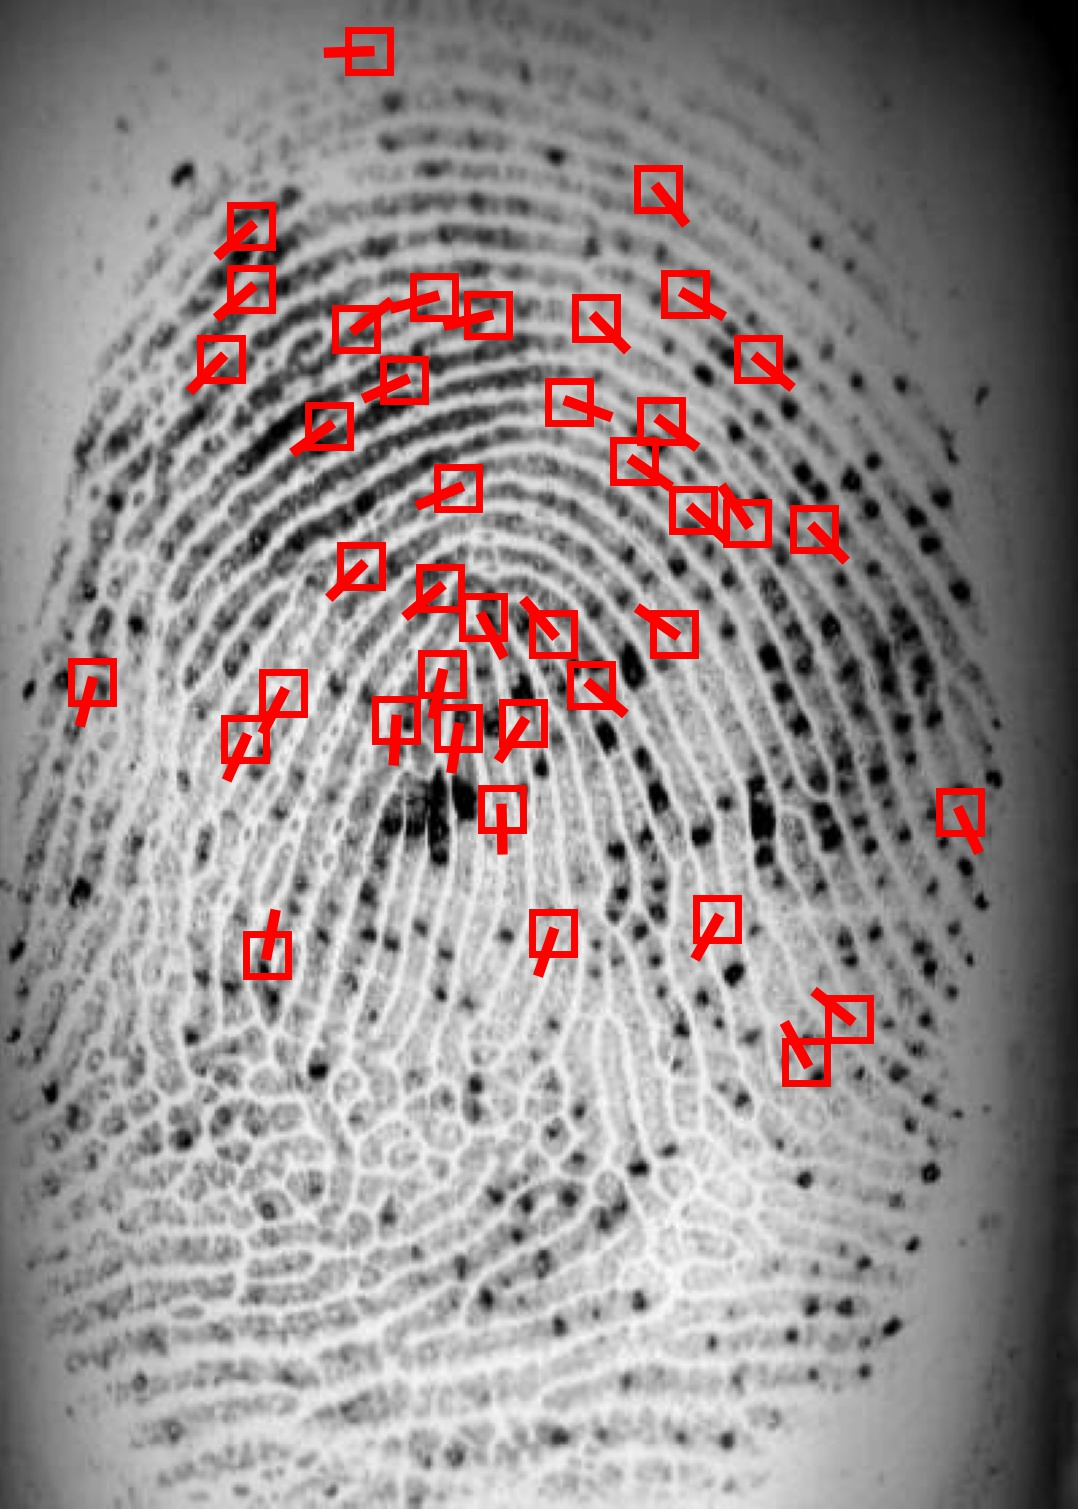
\includegraphics[width=\figwidth\linewidth]{fig/minutiaenet/3.jpg}
    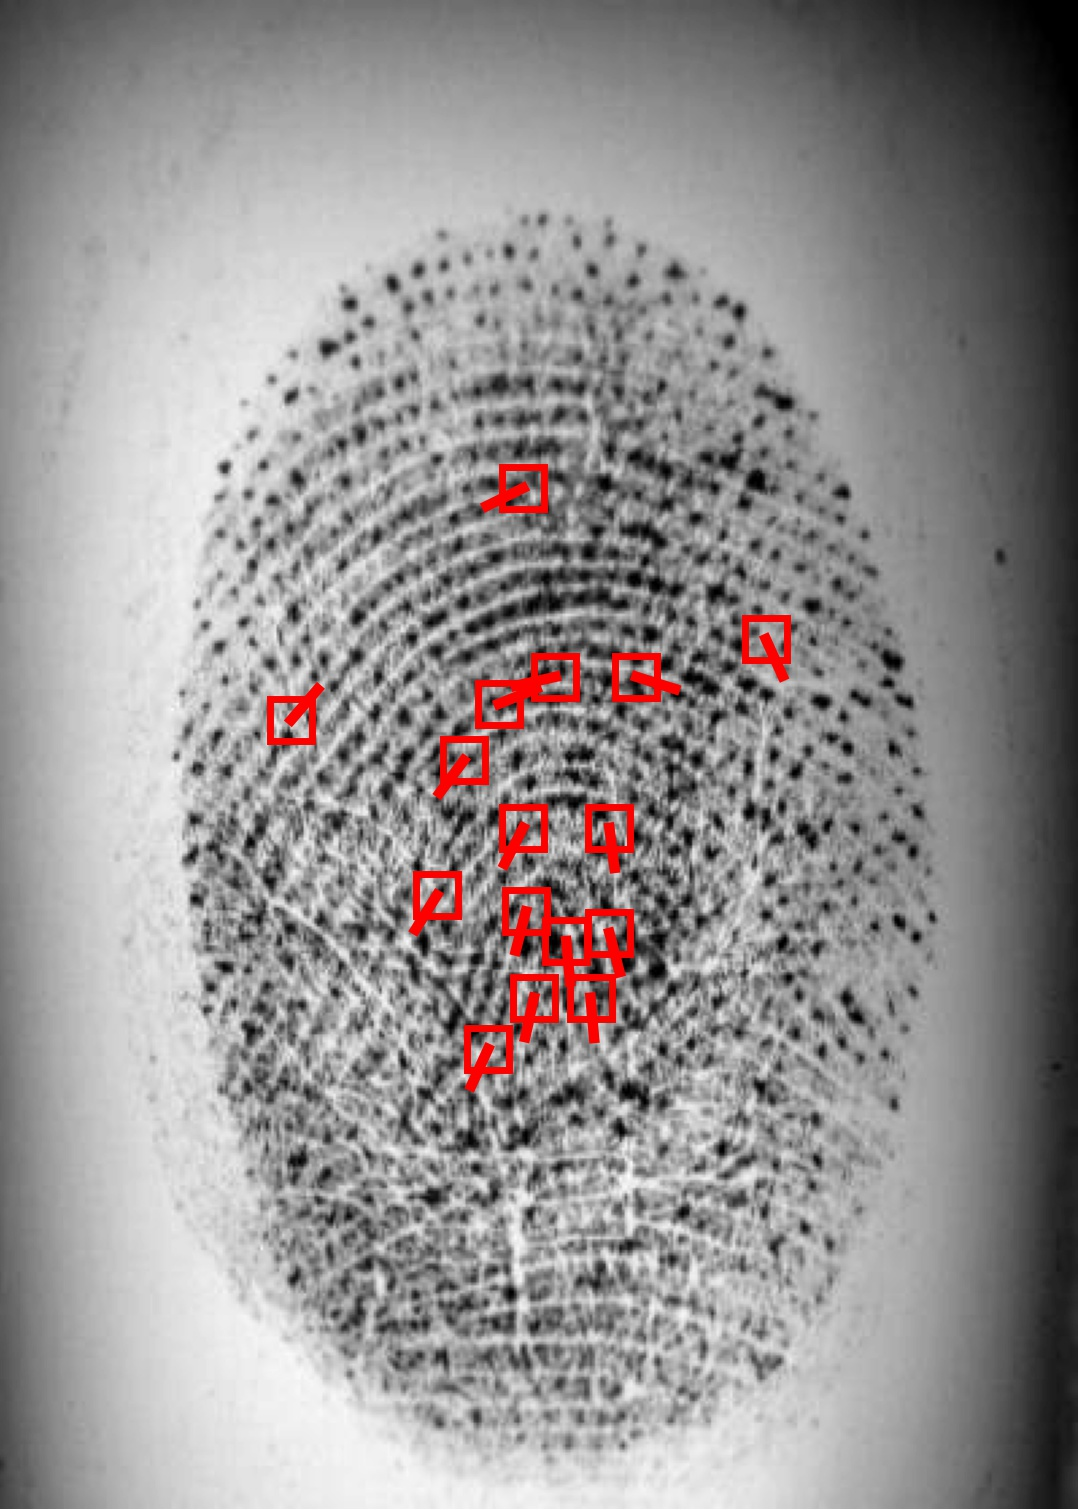
\includegraphics[width=\figwidth\linewidth]{fig/minutiaenet/4.jpg}
    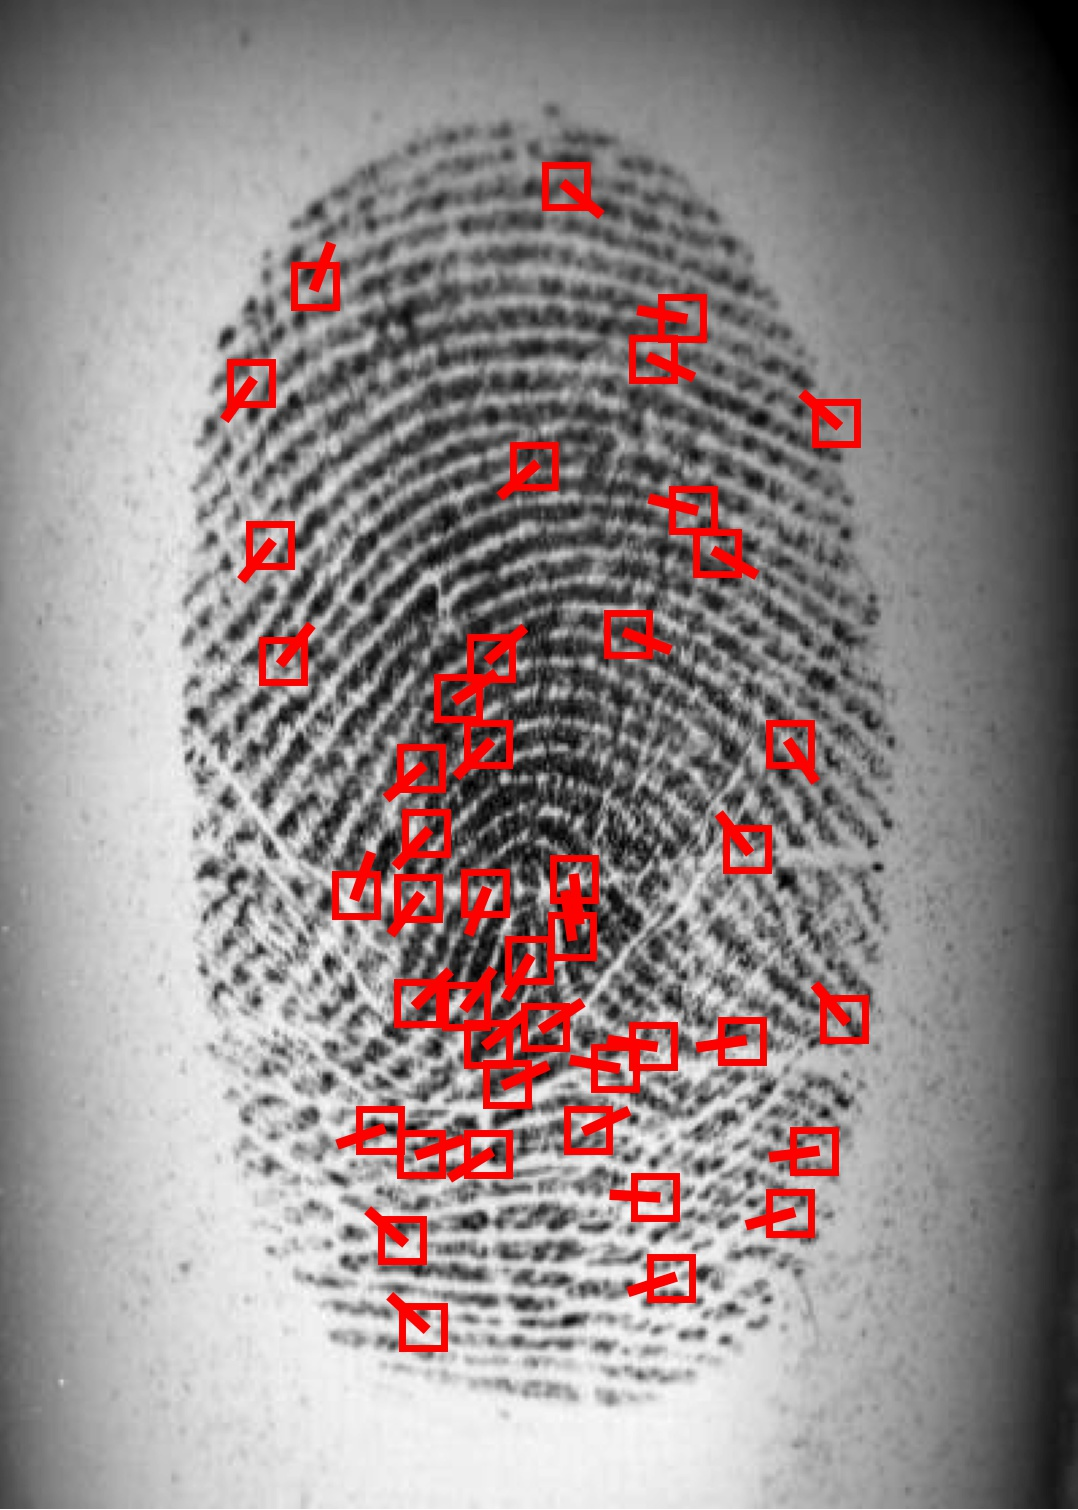
\includegraphics[width=\figwidth\linewidth]{fig/minutiaenet/5.jpg}
    \caption{Some sample minutiae detection results of MinutiaeNet \cite{MinutiaeNet}}
    \label{fig:minutiaenet-results}
\end{figure}

% After detect the minutiae, we then use non maximum suppression to locate the minutiae.

\section{Conclusion and Future Work}


\vspace{1cm}
\begin{table}[htbp]
	\centering
	\caption{Words count}
	\begin{tabular}{l|c}
		\hline
		Abstract & A \\
		Introduction & A \\
		Related Work & A \\
		Methodology & A \\
		Experiments and Results & A \\
		Conclusions and Future Work & A \\ \hline
		Total (exclude references) & A \\ \hline
	\end{tabular}
\end{table}


\bibliographystyle{unsrt}
\bibliography{project-references}

\end{document}
